%%
%%  Department of Electrical, Electronic and Computer Engineering
%%  Chapter 5: Discussion
%%

\chapter{Discussion}
\label{chap_5}

This chapter interprets the results of Chapter~\ref{chap_4} by
considering the experimental findings together
rather than treating each method in isolation.
Several patterns recur across otherwise different experiments,
and these patterns provide a clearer account of where the pose-grouping
problem is constrained
and which changes produce improvements that survive transfer to real data.

Three findings structure the discussion.
First, the experiments with learned grouping heads show that grouping
performance is determined primarily by the quality of the embedding
rather than by the complexity of the downstream read-out.
Second, the synthetic-to-real distribution shift has a larger effect
on the final COCO result than several architectural changes that appear
promising under synthetic-only training.
Third, the end-to-end and detector-swap experiments quantify the
trade-off introduced by separating grouping from detection.
This includes the initially unexpected result that the learned estimate
of the person count can outperform the annotation-level count when
grouping incomplete detector outputs.

The chapter develops these findings using evidence from the successful
and negative experiments reported in Chapter~\ref{chap_4}.
The final section returns to the seven research questions introduced
in Section~\ref{sec_intro_objective}
and summarises the answer to each question together with the
experimental evidence that supports it.

\section{The Embedding Is the Lever}
\label{sec_disc_embedding}

The most consistent finding across the experiments is that pose-grouping
performance depends more strongly on the quality of the per-keypoint
embedding than on the algorithm used to partition those embeddings into
person identities.
This pattern appears across three separate groups of experiments.
Replacing $k$-means with learned grouping heads does not produce
a consistent improvement,
and the more specialised SA-DMoN objective also fails to improve
the underlying representation.
In contrast, changes made directly to the embedding network produce
gains that are retained, and subsequently strengthened, after transfer
to COCO.

This section considers these results together
rather than as independent negative and positive experiments.
The DEC, slot-attention, and graph-partitioning results show what
happens when additional modelling capacity is placed after or alongside
an embedding that still contains ambiguous person assignments.
The SA-DMoN experiments provide a stronger test of the same idea,
by introducing structural information through the clustering objective,
but again fail to move beyond the performance of the simpler baseline.
PG-GAT changes where that structural information enters the pipeline -
instead of asking the grouping head to recover person structure
from the final embeddings,
it uses joint type,
relative geometry,
and same-type relationships during message passing while those
embeddings are being formed.

Taken together, these experiments suggest that the important
distinction is not simply between simple and learned grouping methods
but between introducing structure \emph{after} the representation has
been formed and using that structure to shape the representation itself.
The remainder of this section examines the evidence for this
interpretation
and relates each PG-GAT modification to the failure modes observed
in the earlier grouping-head experiments.

\subsection{Why every learned head failed on the same embedding}
\label{sec_disc_embedding_heads}

Three learned grouping heads, DEC, slot attention, and graph
partitioning, were attached to the standard GAT backbone of
Section~\ref{sec_meth_baseline} and trained jointly with the embedding
under matched optimiser and schedule settings
(Section~\ref{sec_res_learned_heads}).
None produces a grouping result that improves on the no-depth $k$-means
baseline once evaluated on COCO.
The contrast is clearest for graph partitioning -
it is the strongest learned head on synthetic validation at $0.9714$,
but its own COCO read-out falls to $0.7514$.
Applying $k$-means to the embeddings produced by the same jointly
trained model recovers the score to $0.8366$,
which is still below the standard GAT baseline of $0.8841$.
The three heads fail in different ways,
and this consistency across different grouping mechanisms is what makes
the combined result more informative than any individual negative
experiment.

DEC adds little because its clustering objective has limited ability
to correct errors already present in the embedding.
Its KL-divergence objective compares the soft assignment $q$
with a sharpened target $p$ that is itself constructed from $q$
(Equation~\eqref{eq:dec_p_prelim}).
When $k$-means++ initialisation already produces confident assignments,
the target distribution mainly reinforces those assignments rather than
introducing independent supervisory information about person identity.
This behaviour is particularly limiting for the ambiguous cases that
matter most for pose grouping.
If two same-type keypoints from different people lie close together
in embedding space,
an incorrect initial assignment can be sharpened along with the
correct ones.
DEC therefore has no independent structural cue with which to resolve
the error.
This is consistent with its COCO result of $0.8798$,
which remains close to but below the $0.8841$ baseline.

Slot attention behaves differently.
Its synthetic-validation PGA of $0.9025$ exceeds the standard GAT
baseline of $0.8783$,
showing that a learned competitive assignment mechanism can exploit
the relatively clean synthetic representation.
The improvement does not survive transfer -
its own COCO read-out reaches only $0.7986$,
while $k$-means on the jointly trained embeddings reaches $0.8254$.
One limitation is that the slot competition does not explicitly encode
the type-exclusivity constraint available from the pose representation.
Two detections of the same joint type must belong to different people,
but the slot mechanism is not constructed to enforce this relationship
directly.
On the synthetic distribution the embedding can often resolve the
ambiguity without that prior -
the COCO result suggests that this becomes less reliable once the
representation is exposed to the synthetic-to-real shift.
The experiment does not isolate type-exclusivity as the sole cause
of the transfer failure,
but its absence provides a structural explanation consistent with the
observed behaviour.

Graph partitioning provides the strongest example of a synthetic gain
that does not transfer.
Its $0.9714$ synthetic-validation PGA is well above the $0.8783$
baseline,
yet its own COCO grouping falls to $0.7514$.
The $k$-means read-out on the same jointly trained embeddings recovers
to $0.8366$,
indicating that a substantial part of the failure lies in the
partitioning read-out rather than only in the embedding.
The edge classifier converts pairwise affinities into binary decisions,
which are subsequently thresholded and assembled into connected
components.
This creates a sensitivity that is absent from centroid-based $k$-means:
changes in the affinity distribution around the decision threshold
can alter individual edges,
and a small number of incorrect edges can change the connectivity
of an entire component.
The large synthetic-to-COCO deterioration is therefore consistent with
a partitioning mechanism that is particularly sensitive to distribution
shift.

Taken together, the three experiments provide evidence against the
grouping head being the main limitation of the baseline pipeline.
DEC adds an unsupervised sharpening objective,
slot attention introduces a learned competitive assignment mechanism,
and graph partitioning reformulates grouping as supervised pairwise
classification.
Despite these substantially different approaches,
none produces a COCO result above the $0.8841$ $k$-means baseline.
In several cases, applying $k$-means to the jointly trained embeddings
performs better than the head for which those embeddings were trained.

The common result is therefore more important than the individual
failure mechanisms.
Increasing the complexity of the grouping stage does not reliably
recover information that is absent or ambiguous in the representation
supplied to it.
This observation motivates moving the structural priors earlier
in the pipeline,
so that they influence the construction of the embedding itself
rather than being introduced only when that embedding is partitioned.
The SA-DMoN and PG-GAT experiments provide the next two tests
of this interpretation.

\subsection{Why ten SA-DMoN variants plateaued}
\label{sec_disc_embedding_sadmon}

The SA-DMoN experiments extend the grouping-head investigation in a
different direction.
Rather than learning a direct assignment from the final embeddings,
SA-DMoN introduces a graph-structural objective based on modularity
maximisation over the keypoint $k$NN graph.
The ten configurations reported in Section~\ref{sec_res_sadmon}
all converge to a narrow synthetic-validation band of approximately
$0.77$--$0.79$,
around $0.09$ below the no-depth baseline.
More informative than the best individual result is the fact that
substantial changes to the null model,
adjacency,
and type loss do not move the model outside this band.
This suggests that the limitation lies in the compatibility between
the modularity objective and the graph on which it operates
rather than in a particular SA-DMoN hyperparameter.

Newman modularity (Equation~\eqref{eq:newman_modularity}) measures
whether a proposed partition contains more within-community edge mass
than would be expected under a chosen null model.
This formulation is well suited to graphs in which observed connectivity
carries information about the communities of interest,
and the null model provides a reasonable description of connectivity
in the absence of those communities.
The keypoint $k$NN graph is misaligned with this assumption.
Its edges are constructed explicitly from spatial proximity,
whereas the desired partition is person identity.
Two keypoints can therefore be neighbours because they occupy nearby
image coordinates even when they belong to different people.
This occurs precisely in the crowded and overlapping poses for which
grouping is most difficult.

The consequence is a mismatch between the structure emphasised by the
graph and the structure required by the task.
A modularity objective operating on this graph is encouraged to preserve
patterns of local connectivity,
but those patterns need not correspond to person identity.
In crowded scenes they may instead connect joints belonging to different
people.
The spectral objective is therefore being asked to recover identity
communities from a graph whose edges were not constructed primarily
from identity information.
This provides a structural explanation for why changing the details
of the modularity formulation has little effect on the final grouping
accuracy.

The SA-DMoN variants test this explanation from several directions.
Changing the spatial bandwidth $\sigma$ modifies how strongly proximity
enters the skeleton-aware null model,
but no tested parameterisation produces a useful operating point.
With unconstrained optimisation, $\sigma$ grows to approximately $341$,
making the spatial kernel nearly uniform and effectively weakening
the intended spatial correction.
Constraining $\sigma$ to $[0.05,0.5]$ prevents this divergence,
but the learned value moves to the upper boundary,
again indicating that the optimisation prefers a weaker spatial null.
Fixing $\sigma$ from the per-graph median pairwise distance moves
in the opposite direction and also reduces performance.
The behaviour across these variants is more consistent with a poorly
matched objective than with a single badly chosen bandwidth.

The v2 experiments alter other parts of the formulation but reach the
same conclusion.
Feature-based adjacency breaks the direct dependence between the
message-passing graph and the spatial null
but makes the adjacency itself change as the representation is learned.
The modularity objective must then optimise against a graph that is
moving with the embedding.
Reducing the spectral weight partially recovers the loss in performance
but does not exceed the earlier variants.
Replacing the hinge-style type term with an entropy formulation changes
the smoothness of the optimisation without changing the information
available to the objective,
and similarly produces no meaningful gain.
Combining the two changes does not improve the result.

The narrow performance range across all ten configurations is therefore
the main evidence from the SA-DMoN investigation.
It does not establish that modularity objectives are unsuitable for pose
grouping in general -
a graph whose edges encode learned identity affinity rather than
spatial proximity could behave differently.
It does show that, for the keypoint $k$NN graph used here,
increasingly elaborate modifications to the modularity objective do not
recover the performance of the simpler contrastive-embedding baseline.

Together with the learned-head experiments,
this result substantially narrows the useful design space.
The earlier experiments show that DEC,
slot attention,
and pairwise graph partitioning do not reliably improve grouping once
the representation transfers to COCO.
SA-DMoN then shows that introducing pose structure through a
modularity-based clustering objective does not resolve the problem either.
These results motivate moving the structural information into the
representation-learning stage itself.
PG-GAT follows this direction by retaining the simple $k$-means read-out
and instead changing how information is exchanged between keypoints
while their embeddings are being formed.

\subsection{Why the three PG-GAT modifications are complementary}
\label{sec_disc_embedding_pggat}

The PG-GAT isolation ablation of
Section~\ref{sec_res_pggat_ablations} tests each of the three
skeleton-aware modifications independently before combining them in the
full model.
The three individual configurations are tightly grouped on synthetic
validation at $0.8825$,
$0.8825$, and $0.8834$,
compared with $0.8783$ for the standard GAT baseline.
Enabling all three modifications increases PGA to $0.8896$,
which is $0.0062$ above the strongest individual configuration
and $0.0113$ above the baseline.
The individual differences are small enough that they should not be
interpreted as a ranking of the three mechanisms.
The more useful result is that no single modification accounts for the
performance of the full model.
Their combination produces a larger improvement than any modification
in isolation,
consistent with the three mechanisms providing complementary rather
than redundant information.

This interpretation follows from the different roles of the three
modifications.
The type-pair attention bias introduces learnable additive terms for
the four edge categories used by PG-GAT:
same-type,
skeletal-neighbour,
same-limb,
and cross-body.
In the standard GATv2 formulation,
attention is derived from the features of the incident nodes and does
not explicitly distinguish these structural relationships.
The type-pair term makes the edge category available directly to the
attention calculation,
allowing otherwise similar node pairs to receive different attention
biases according to their relationship in the pose graph.

The skeleton-aware position encoding provides a complementary source of
information.
It exposes L2 distance,
skeleton-hop distance,
and the same-type indicator directly to the attention mechanism.
Although absolute position is already present in the node representation,
a standard GATv2 layer must infer relative geometric relationships
through the interaction between the two node features.
Providing these relationships explicitly reduces the burden on the
attention layer and,
in the case of skeleton-hop distance,
introduces information that cannot be recovered from image coordinates
alone.

The repulsion mechanism addresses a narrower problem.
One of the four attention heads is restricted to same-type edges,
concentrating part of the model capacity on comparisons such as
left-wrist against left-wrist or right-knee against right-knee.
These are particularly informative for person separation because two
detections of the same joint type cannot belong to the same person.
The dedicated head therefore gives the network a separate pathway
in which the contrastive objective can act on the subset of
relationships most directly associated with cross-person discrimination.

The isolation results are consistent with these three mechanisms being
complementary.
Type-pair attention contributes categorical edge structure,
position encoding contributes relative geometric and topological
information,
and the repulsion head reserves capacity for same-type discrimination.
Their individual gains are modest,
but the combined configuration performs better than any of them alone.
Given that these are single-run measurements and the individual
differences are close to the observed run-to-run variation,
the ablation does not establish the precise interaction between their
gradients.
It does, however, support retaining all three modifications in the
architecture that is subsequently taken into the Bayesian sweep.

The architecture sweep then produces a much larger improvement than any
of the isolation changes.
Starting from the full two-layer PG-GAT configuration at $0.8896$,
the sweep over network depth,
attention-head count,
hidden dimension,
output dimension,
joint-type embedding dimension,
and dropout selects a three-layer configuration with a $256$-dimensional
output and reaches $0.9634$ synthetic-validation PGA.
This is an increase of $0.0738$ over the matched-architecture ablation
configuration.
By comparison, the subsequent loss sweep does not find a configuration
that meaningfully exceeds the inherited contrastive settings -
its best result of $0.9617$ is slightly below the architecture-sweep
winner.

The relative scale of these effects gives a more complete interpretation
of the PG-GAT result.
The skeleton-aware modifications provide the inductive biases that
distinguish PG-GAT from the standard GATv2 baseline,
but their benefit depends strongly on the architecture in which they
operate.
The two-layer isolation experiment establishes that the modifications
provide a useful signal at matched compute,
while the architecture sweep shows that considerably more of that signal
can be exploited with an additional layer and a larger embedding space.
In contrast, varying the contrastive margin,
number of repulsion heads,
learning rate,
and weight decay does not produce a comparable gain.

The main lever is therefore not a more elaborate grouping objective
or a finely tuned loss
but the combination of task-specific structure and sufficient
representation capacity.
PG-GAT introduces information that the standard GATv2 formulation does
not expose explicitly,
and the architecture sweep identifies a network size that makes better
use of that information.
The loss sweep, in turn, provides evidence that the improvement is not
primarily the result of a favourable choice of contrastive
hyperparameters.
This distinction is important when interpreting the headline model -
its performance is not attributable to a single architectural
modification or tuned loss value
but to the combination of skeleton-aware message passing and an
architecture sized to exploit it.

\subsection{Synthesis}
\label{sec_disc_embedding_synthesis}

Reading Sections~\ref{sec_disc_embedding_heads}--\ref{sec_disc_embedding_pggat}
together gives a consistent picture of where the main performance
constraint lies.
The learned grouping heads fail for different reasons,
yet none improves on the simple $k$-means baseline after transfer to
COCO.
The SA-DMoN experiments reach the same conclusion from a graph-structural
direction -
changing the null model,
adjacency,
spectral weight,
and type-loss formulation does not overcome the mismatch between
modularity and the spatial $k$NN graph.
In contrast, modifying the embedding network itself produces a measurable
improvement at matched architecture and a much larger gain once the
architecture is sized by the Bayesian sweep.

The evidence therefore identifies the embedding network as the stronger
lever for pose-grouping performance in the setting studied here.
This does not imply that the grouping algorithm is irrelevant
or that a different grouping formulation could never improve the result.
Rather, within the range of grouping methods evaluated in this work,
additional complexity at the read-out stage contributes less than
improving the representation that the read-out receives.
The effectiveness of $k$-means in the final pipeline follows from this
result -
once the embedding separates person identities sufficiently well -
a simple partitioning method is adequate and avoids introducing another
learned component whose behaviour must transfer across domains.

This provides the experimental answer to \emph{RQ1: the lever}.
For the pose-grouping formulation and data considered in this work,
the main opportunity for improvement lies in the construction of the
per-keypoint embedding rather than in replacing its downstream grouping
algorithm.
This finding also motivates the later experiments in the chapter,
which retain $k$-means and investigate how the representation behaves
under domain transfer,
alternative geometries,
and detector-independent evaluation.

The PG-GAT ablation and architecture sweep provide the corresponding
answer to \emph{RQ2: inductive biases}.
Type-pair attention,
skeleton-aware position encoding,
and same-type repulsion each produce a small positive change when
introduced independently at the matched baseline architecture.
Their combination gives the strongest isolation result,
indicating that the three sources of pose structure are complementary
at the resolution of the experiment.
The architecture sweep then shows that the benefit of these inductive
biases depends strongly on the capacity of the network that uses them,
selecting a three-layer,
$256$-dimensional configuration that substantially outperforms the
two-layer ablation model.

Taken together, RQ1 and RQ2 establish the design basis for the
remainder of the discussion.
The first identifies \emph{where} additional modelling effort is most
productive -
the embedding rather than the grouping head.
The second identifies \emph{how} that embedding can be improved -
by exposing pose-specific categorical,
geometric,
and same-type relationships directly to the attention mechanism
and providing sufficient representation capacity to use them.
The subsequent COCO fine-tuning and end-to-end experiments test whether
these gains remain useful once the model leaves the synthetic
distribution on which these design decisions were developed.

\section{What Survives Synthetic-to-Real, and What Does Not}
\label{sec_disc_transfer}

The second cross-cutting finding is that the synthetic-to-real
distribution shift is one of the strongest determinants of performance
in this work.
Several configurations that perform well, or appear promising, on the
synthetic distribution lose part or all of that advantage when evaluated
on COCO.
Conversely, the largest improvement in the experimental chapter comes
not from introducing another architectural mechanism,
but from adapting the selected PG-GAT model to the COCO distribution
through fine-tuning.

This pattern appears across several experiments that otherwise have
little in common.
Removing the depth channel reduces synthetic performance but improves
zero-shot COCO transfer.
Fine-tuning PG-GAT on COCO produces a substantially larger improvement
than any individual PG-GAT modification.
The reduced-dimensional hyperbolic representation is competitive in the
synthetic-only setting but does not retain that advantage after COCO
fine-tuning.
TriGAT introduces articulation information that is meaningful in
principle,
yet performs worse after transfer,
while the visual-feature variant adds appearance information without
improving on the final position-and-type-only PG-GAT.
These experiments alter different parts of the pipeline,
but each exposes the same underlying difficulty -
a representation that is useful on the synthetic distribution is not
necessarily the representation that transfers best to real keypoint data.
Figure~\ref{fig:transfer_scatter} shows the pattern across every configuration in
Chapter~\ref{chap_4} that reports both numbers.

\begin{figure}[H]
    \centering
    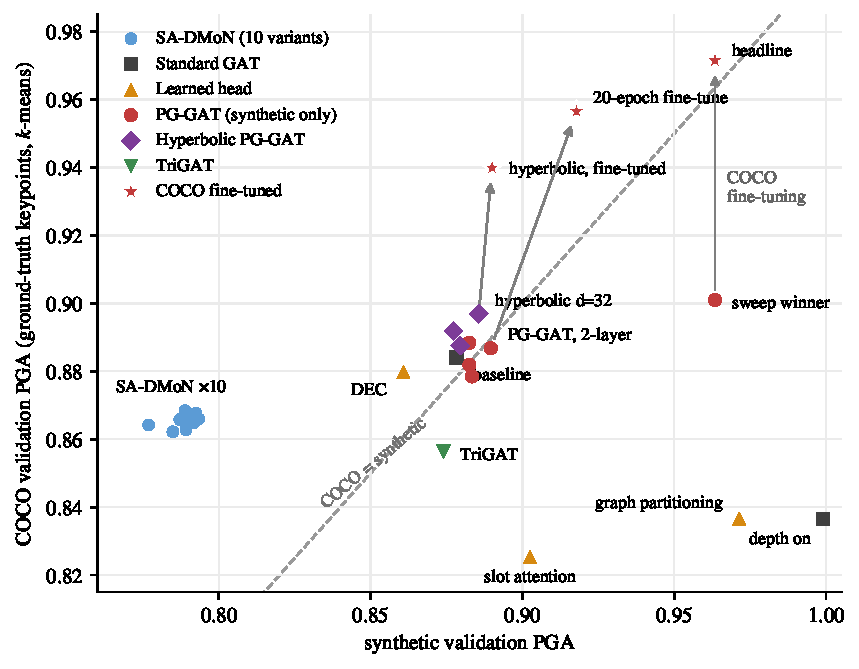
\includegraphics[width=0.92\linewidth]{figures/transfer_scatter.pdf}
    \caption[Synthetic-validation against COCO-validation PGA across the evaluated configurations.]{Synthetic-validation PGA against COCO-validation PGA
    using ground-truth keypoints and $k$-means
    for the 27 configurations in Chapter~\ref{chap_4} that report both metrics.
    The dashed diagonal represents equal performance on the two datasets;
    points below it perform worse on COCO than on the synthetic validation set,
    with the vertical distance from the diagonal indicating the transfer gap.
    Arrows connect the three synthetic-only models to their corresponding COCO fine-tuned versions,
    showing the change produced by real-data adaptation.
    Values are taken directly from the results reported in Chapter~\ref{chap_4}.
    TriGAT is evaluated on the $2{,}180$ scenes containing valid triplets,
    while all other configurations are evaluated on $2{,}307$ scenes.}
    \label{fig:transfer_scatter}
\end{figure}

The evidence therefore suggests that synthetic validation should be
treated primarily as a controlled environment for developing and
isolating architectural ideas,
rather than as a reliable predictor of their final COCO performance.
This distinction is important because the synthetic data remains useful
throughout the investigation.
It provides known person identities,
controlled scene composition,
and a repeatable setting in which individual design changes can be
compared without the additional variation introduced by a real detector.
The limitation is not that synthetic evaluation is uninformative,
but that improvements measured there cannot automatically be interpreted
as improvements in real-data grouping.

The remainder of this section examines this transfer effect through the
depth-removal experiment,
the COCO fine-tuning results,
and the hyperbolic,
TriGAT,
and visual-feature variants.
Considered together, these experiments show both sides of the same
problem -
features that make the synthetic task easier can become liabilities
after transfer,
while relatively modest adaptation to the target distribution can
produce larger gains than substantial changes to the model itself.
This distinction between \emph{synthetic discriminability} and
\emph{transferable discriminability} is central to interpreting the
experimental results that follow.

\subsection{Depth removal: the diagnostic that exposed the shift}
\label{sec_disc_transfer_depth}

The depth-removal diagnostic of Section~\ref{sec_res_baseline} provides
the clearest early evidence of the synthetic-to-real distribution shift.
With depth included, the standard GAT reaches a synthetic-validation
PGA of $0.9990$ but transfers to COCO at only $0.8366$.
Removing the depth channel reduces synthetic-validation PGA to $0.8783$,
a drop of $0.1207$,
while increasing COCO PGA to $0.8841$,
a gain of $0.0475$.
The direction of the two changes is more informative than either number
alone -
the feature that makes the synthetic grouping problem almost trivial is
also the feature that produces the weaker real-data representation.

The explanation lies in how depth is obtained in the two domains.
The synthetic generator of Section~\ref{sec_meth_data_synth} provides
metric depth from the Blender scene,
whereas the COCO pipeline of Section~\ref{sec_meth_data_coco} estimates
depth using MiDaS~\cite{ranftl2020midas}.
The latter provides relative depth rather than a metric camera-space
coordinate,
with scale and calibration that can vary between images.
A model trained on the synthetic depth channel can therefore exploit
relationships that are highly stable in the rendered data,
but are not represented in the same way at COCO inference time.
Removing depth sacrifices this particularly strong synthetic cue,
but also removes a source of distribution mismatch.

This result also explains why the depth-on synthetic configuration is a
poor setting in which to evaluate subsequent embedding modifications.
At $0.9990$ PGA there is almost no remaining grouping error for a new
architectural mechanism to correct.
The model can rely heavily on the metric depth coordinate to separate
people in three-dimensional scenes,
leaving little room for changes to the attention mechanism to produce a
measurable improvement.
Removing depth makes the synthetic problem harder,
but in doing so produces a more useful experimental setting for studying
whether the embedding network can learn person separation from signals
that are also available consistently on real data.

The depth-removal experiment therefore serves two purposes in the
methodology.
First, it motivates the no-depth configuration used by the subsequent
PG-GAT experiments.
Second, it establishes an important distinction for interpreting the
remainder of the results,
making the synthetic task easier is not equivalent to learning a
representation that transfers better.
A synthetic improvement is useful evidence only when the mechanism
responsible for that improvement remains meaningful under the
corresponding real-data distribution.
The experiments that follow repeatedly return to this distinction.

\subsection{COCO fine-tune: the largest lift in the pipeline}
\label{sec_disc_transfer_finetune}

The COCO fine-tuning experiment of Section~\ref{sec_res_coco_ft}
provides the clearest measurement of how strongly the target-data
distribution affects the final grouping result.
The synthetic-pretrained architecture-sweep winner reaches $0.9010$
COCO val PGA before fine-tuning and $0.9715$ after the fine-tune sweep,
an improvement of $0.0705$ on the same PG-GAT architecture.
This gain is substantially larger than the approximately $0.011$
improvement produced by combining the three PG-GAT modifications
at the matched baseline architecture
(Section~\ref{sec_disc_embedding_pggat}),
and is comparable in magnitude to the $0.0738$ improvement obtained
from the architecture sweep itself.
Adaptation to the target distribution is therefore one of the largest
individual effects measured in the experimental chapter.

Two aspects of this result help explain its significance.
First, the COCO improvement does not come at the expense of the
synthetic representation.
The fine-tuned checkpoint retains a synthetic-validation PGA of
$0.9634$,
equal to the value measured for the architecture-sweep checkpoint
before fine-tuning.
The corresponding synthetic-test result of $0.9580$ provides the same
general picture.
Within the resolution of these measurements,
the fine-tune therefore adapts the representation to COCO without
removing the person-separation structure learned during synthetic
pre-training.
The two stages appear complementary rather than competitive,
synthetic training establishes a useful grouping representation,
and COCO fine-tuning adjusts that representation to the statistics
of the target domain.

Second, relatively little additional performance is obtained by
optimising the fine-tuning recipe itself.
A 20-epoch fine-tune of the architecture-sweep winner reaches $0.9695$
COCO val PGA,
while the 12-run Bayesian sweep improves this to $0.9715$.
The difference of $0.0020$ is small relative to the variation of the
metric and should not be interpreted as a substantive gain.
Instead, the sweep shows that the inherited recipe lies within a
relatively flat region of the fine-tuning search space.
Its main contribution is therefore to support the choice of learning
rate,
weight decay,
and training duration rather than to provide another major source
of performance.

The contrast between these two effects is informative.
Changing the model's exposure from synthetic-only training to COCO
fine-tuning produces a $0.0705$ gain,
whereas searching over reasonable ways of performing that fine-tuning
produces only a further $0.0020$.
The important variable is therefore the target-domain data itself,
rather than a narrowly tuned optimisation schedule.
This reinforces the interpretation of the depth experiment -
representations learned from synthetic data can provide a strong
starting point,
but their final real-data performance depends heavily on whether the
information they encode remains appropriate for the target distribution.

This result provides the reference point for the architectural variants
considered next.
Hyperbolic embedding,
the triplet representation,
and visual-feature augmentation each introduce additional
representational structure that could, in principle, improve person
separation.
Their value cannot be judged from synthetic performance alone, however.
The more demanding question is whether the additional structure produces
an advantage once the model is evaluated or adapted on the real-data
distribution.
The results of those experiments show that this condition is
considerably harder to satisfy.

\subsection{Hyperbolic Option~B: the geometric prior loses to fine-tuning}
\label{sec_disc_transfer_hyperbolic}

The hyperbolic PG-GAT experiments of Section~\ref{sec_res_hyperbolic}
provide a useful example of an advantage that appears under
synthetic-only training but does not survive adaptation to the target
distribution.
Under H2, a $32$-dimensional hyperbolic embedding reaches $0.8856$
synthetic-validation PGA,
compared with $0.8896$ for the $128$-dimensional Euclidean ablation
model.
The difference is small relative to the variation of the metric,
so the result supports the intended efficiency interpretation -
in this setting, the hyperbolic representation retains approximately
the same grouping quality with a four-fold reduction in embedding
dimension.

The important test is whether that dimensional advantage persists once
the models are exposed to COCO.
Option~B fine-tunes the $32$-dimensional hyperbolic model and reaches
$0.9399$ COCO val PGA.
This is substantially higher than its synthetic-only COCO transfer
result of $0.8969$,
showing that the hyperbolic representation also benefits from
target-domain adaptation.
The improvement is not enough, however, to make it competitive with
the strongest Euclidean configurations.
It remains below the $0.9565$ legacy Euclidean fine-tune result and
$0.0316$ below the sweep-selected Euclidean headline of $0.9715$.
The dimensional efficiency observed in the synthetic-only experiment
therefore does not translate into a competitive fine-tuned COCO result.

One possible explanation is the scale of the hierarchy represented by
the pose graph.
The theoretical motivation for hyperbolic embeddings is strongest for
hierarchical and tree-like structures whose number of nodes grows
rapidly with depth,
where Euclidean representations require increasing dimension to
represent the structure with low distortion~\cite{sarkar2011treeembed}.
The COCO skeleton is small by comparison -
it contains only $17$ joint types and has a maximum topological depth
of only a few hops.
The pose-grouping problem may therefore provide too little hierarchical
structure for the geometric advantage of hyperbolic space to become
large at the embedding dimensions considered here.
This interpretation is consistent with the dim-$32$ result,
where hyperbolic geometry appears to preserve useful structure
efficiently,
but does not create a higher-quality representation than the larger
Euclidean model.

The fine-tuning results expose a second and empirically stronger effect.
The Euclidean PG-GAT gains $0.0705$ COCO PGA when the architecture-sweep
checkpoint is adapted from synthetic-only training to the final
COCO-fine-tuned configuration.
The hyperbolic Option~B model also improves after fine-tuning,
but its gain is smaller -
$0.8969$ to $0.9399$, or $0.0430$.
Whatever representational advantage the hyperbolic geometry provides
at low dimension is therefore not sufficient to compensate for the
stronger target-domain performance reached by the Euclidean model.
The experiment does not isolate whether this difference is caused by
embedding dimension,
manifold geometry,
optimisation behaviour,
or an interaction between them,
but it does establish that the synthetic efficiency result alone is not
predictive of the final COCO ranking.

The two pre-registered hypotheses should consequently be interpreted
separately.
H1, which predicts a quality advantage for hyperbolic embedding at
comparable dimension, is not supported by the experiments.
H2 receives partial support -
the $32$-dimensional hyperbolic model approximately matches the
$128$-dimensional Euclidean ablation model under synthetic-only training,
demonstrating that useful grouping structure can be represented at
substantially lower dimension.
That advantage does not survive strongly enough after COCO fine-tuning
to produce a competitive final model.
Hyperbolic PG-GAT is therefore best viewed as an efficiency observation
under the synthetic regime,
rather than as an alternative to the Euclidean headline configuration.

\subsection{TriGAT: a richer primitive whose downstream voting step is lossy}
\label{sec_disc_transfer_trigat}

TriGAT (Section~\ref{sec_res_trigat}) explores a different alternative
to the standard PG-GAT formulation.
Rather than changing the embedding geometry or adding another feature
source, it changes the graph primitive from individual joints to
triplets of three connected joints.
The motivation is that a triplet provides local articulation information
through its pivot angle,
which is invariant to global rotation and is not directly available
from the position of a single joint.
Under the matched synthetic training regime, however,
TriGAT reaches $0.8740$ synthetic-validation PGA compared with $0.8896$
for the corresponding PG-GAT ablation configuration,
a difference of $-0.0156$.

The main weakness of the implemented formulation appears in the
conversion from triplet-level clusters back to joint-level assignments.
A joint can belong to several overlapping triplets,
and those triplets are not guaranteed to receive the same cluster label
after $k$-means.
The weighted-majority rule of Section~\ref{sec_meth_trigat_voting}
must therefore reconcile potentially inconsistent triplet assignments
before the final joint partition can be formed.
This introduces an additional inference step that is absent from the
joint-based PG-GAT pipeline.

Errors at the triplet level can also propagate through this conversion.
A mis-clustered triplet contains three joints and overlaps with
neighbouring triplets,
so its incorrect assignment can influence the final labels of several
joints.
The voting rule can correct an isolated error when the remaining
triplets agree,
but it cannot recover reliably when several overlapping assignments
disagree.
The additional articulation information must therefore provide enough
improvement in the triplet embedding to compensate for the error
introduced by the subsequent voting stage.
The measured result indicates that this does not happen in the present
architecture.

This result does not show that articulation is an unhelpful cue.
The triplet representation explicitly contains pivot-angle information
that is absent from the single-joint input,
and the pivot angle is a rotation-invariant descriptor of local
articulation.
Instead, the experiment shows that the implemented route for exploiting
this information loses more during the triplet-to-joint conversion than
it gains from the richer representation.
The negative result therefore applies to the combination of triplet-level
embedding,
triplet-level clustering,
and joint-level voting rather than to the articulation signal itself.

A natural follow-on would be to retain the articulation information
while avoiding the intermediate triplet clustering.
For example, overlapping triplet embeddings could be aggregated into a
joint-level representation before clustering,
or a learned mapping could predict joint assignments directly from the
surrounding triplet representations.
Either approach would preserve the joint as the final grouping primitive
while still allowing local articulation to contribute to its embedding.
These alternatives require a different architecture and are therefore
left for future work.

The TriGAT experiment consequently answers the graph-primitive question
more narrowly than a simple comparison between joints and triplets might
suggest.
Changing to a richer primitive does not improve grouping merely because
that primitive contains additional information -
the architecture must also preserve that information through to the
final joint-level decision.
For the TriGAT formulation evaluated here,
the evidence points to the triplet-to-joint voting stage as the main
bottleneck,
making the implemented design a documented negative result rather than
evidence against articulation-based features more generally.


\subsection{PG-GAT v2: visual features do not beat the sweep-defended baseline}
\label{sec_disc_transfer_v2}

The PG-GAT v2 experiment tests whether appearance information can add
useful identity cues beyond the position-and-type representation used by
the standard PG-GAT (Section~\ref{sec_res_v2}).
Pre-trained MobileNetV2 features are sampled at each keypoint location
and projected into the node representation before message passing.
The 20-epoch configuration reaches $0.9670$ COCO val PGA,
while extending training to 50 epochs raises this to $0.9682$.
Both remain below the \texttt{meng-headline} result of $0.9715$,
by $0.0045$ and $0.0033$ respectively.
The additional visual information therefore does not produce a better
operating point in the configuration evaluated here.

This result is consistent with the diminishing returns observed in the
earlier feasibility experiments.
When MobileNetV2 features were added to a simple position-based
$k$-means representation, the improvement was approximately $+0.07$
COCO PGA.
As the underlying representation became stronger, however,
the additional gain from the same visual signal became much smaller.
This suggests that appearance features are most useful when the existing
representation contains relatively little identity information.
Once position, joint type, skeleton structure, and learned message
passing already provide a strong separation between people, much of the
useful information supplied by the visual features may be redundant.

The fully trained v2 experiment follows this pattern.
PG-GAT already uses joint type and relative skeleton structure to
organise the embedding,
and COCO fine-tuning adapts that representation directly to the target
distribution.
At this operating point, adding generic ImageNet features does not
improve the final PGA.
This does not imply that the visual features contain no identity
information - the earlier feasibility result shows that they do.
Rather, their marginal contribution decreases as the non-visual
embedding becomes stronger.
The additional signal is not sufficient to produce an improvement over
the sweep-selected and COCO-fine-tuned PG-GAT configuration.

There is an important qualification to this comparison.
PG-GAT v2 extends the legacy two-layer architecture rather than the
architecture-sweep-selected three-layer headline model.
The experiment therefore does not isolate the marginal effect of adding
visual features to the exact \texttt{meng-headline} architecture.
A fully matched ablation would require adding the same visual pathway
to the sweep-selected PG-GAT and repeating the fine-tune procedure.
The present result supports the narrower conclusion that the implemented
v2 configuration does not provide a better practical operating point
than the final position-and-type model -
it does not establish that visual features could never improve a
stronger or differently trained PG-GAT.

The computational cost makes the measured trade less attractive.
The v2 network contains approximately $27{,}000$ additional parameters
relative to the legacy two-layer PG-GAT that it extends,
and the frozen MobileNetV2 feature extractor contributes a further
approximately $2.2 \times 10^{6}$ parameters.
More importantly, the MobileNetV2 backbone must be executed at
inference time because its feature maps are required to construct the
visual node features.
When combined with the HigherHRNet detector and PG-GAT v2 network,
the resulting deployable pipeline contains approximately
$31.0 \times 10^{6}$ parameters,
compared with approximately $28.6 \times 10^{6}$ for HigherHRNet alone.

The added computation is not accompanied by an accuracy gain in the
experiments reported here.
The extended v2 configuration reaches $0.9682$ COCO val PGA,
below the $0.9715$ no-visual-feature PG-GAT headline.
The HigherHRNet AE figure of $0.9847$ is also higher,
although that value is an end-to-end PGA measured on matched detector
outputs and should not be treated as a strictly like-for-like comparison
with the ground-truth-keypoint v2 value.
It is nevertheless relevant to the deployment trade -
the visual pathway increases the total system size without closing the
accuracy gap to the native detector-specific grouping mechanism.

The experiment therefore provides a negative result for the visual
augmentation implemented in PG-GAT v2.
Appearance features are useful when added to a weak positional
representation,
but their marginal value decreases as the underlying embedding improves.
At the operating points tested here,
the additional MobileNetV2 pathway increases model size and inference
requirements without exceeding the simpler PG-GAT headline.
For that reason, visual augmentation is not pursued further in this
work.
A future investigation could revisit the idea using a matched
sweep-selected architecture,
detector-native visual features,
or jointly trained appearance features,
but those experiments would test a different formulation from the frozen
ImageNet feature pathway evaluated here.

\subsection{Synthesis}
\label{sec_disc_transfer_synthesis}

Reading Sections~\ref{sec_disc_transfer_depth}--\ref{sec_disc_transfer_v2}
together shows that the synthetic-to-real shift affects each of the
alternative representations in a different way.
The depth-on baseline is the clearest example -
near-perfect synthetic performance falls to $0.8366$ on COCO because
the depth signal changes between the two domains.
The low-dimensional hyperbolic model retains useful structure
efficiently under synthetic training,
but its advantage is not sufficient to remain competitive after COCO
fine-tuning.
TriGAT introduces articulation information but loses more through its
triplet-to-joint voting stage than it gains from the richer primitive.
The visual-feature variant adds appearance information at considerable
computational cost,
yet the implemented configuration remains below the
position-and-type-only headline model.
Although the mechanisms differ, the common result is that an advantage
observed or motivated in the controlled setting does not automatically
translate into an advantage at the final COCO operating point.

The COCO fine-tuning experiment provides the strongest counterpoint.
Adapting the architecture-sweep-selected PG-GAT from synthetic training
to COCO increases COCO val PGA from $0.9010$ to $0.9715$,
a gain of $0.0705$,
while preserving its $0.9634$ synthetic-validation PGA.
This improvement is comparable to the gain produced by the architecture
sweep itself and larger than the changes associated with the individual
architectural alternatives considered in this section.
The result therefore identifies exposure to the target distribution
as a major determinant of real-data grouping performance,
rather than treating synthetic performance as a sufficient proxy for it.

This provides the experimental answer to \emph{RQ6: synthetic-to-real
transfer}.
Synthetic data provides a useful environment for isolating architectural
effects and learning an initial person-separation representation,
but performance measured there is not by itself a reliable predictor
of the final COCO ranking.
Features that are highly discriminative in the synthetic domain can
transfer poorly when their statistics change,
as demonstrated most directly by depth.
Conversely, a representation that is already strong on synthetic data
can still gain substantially when adapted to the target distribution.
The synthetic and real stages should therefore be treated as complementary,
the former supports controlled architectural development,
while the latter is necessary to establish whether the resulting
representation remains useful under realistic data.

This finding also constrains the answers to \emph{RQ4: embedding
geometry} and \emph{RQ5: graph primitive}.
For RQ4, the hyperbolic experiments provide evidence that a
lower-dimensional representation can retain comparable grouping
information under synthetic-only training,
but they do not establish a quality advantage over the Euclidean
embedding at the final COCO operating point.
The result is therefore best interpreted as an efficiency observation,
rather than as evidence for replacing the Euclidean headline model.
For RQ5, the TriGAT result shows that introducing articulation through
a triplet primitive does not improve grouping in the architecture
evaluated here.
The negative result is associated with the additional triplet-clustering
and voting stage,
rather than demonstrating that articulation itself is uninformative.

The visual-feature experiment provides a related negative result.
The implemented MobileNetV2 augmentation reaches $0.9682$ COCO val PGA,
compared with $0.9715$ for the no-visual-feature headline model,
while requiring an additional visual feature extractor at inference.
Because the v2 experiment uses the legacy two-layer architecture rather
than the sweep-selected headline architecture,
it does not isolate the marginal effect of appearance features on the
final PG-GAT configuration.
It does, however, show that the implemented visual pathway does not
provide a better practical operating point than the simpler
position-and-type model.

The methodological consequence is not that architectural alternatives
are unimportant,
but that they must be judged after the relevant domain shift rather
than by their synthetic behaviour alone.
In the experiments reported here, the most reliable path to the final
result is to retain the skeleton-aware PG-GAT representation selected
by the architecture sweep and then adapt that representation to COCO.
The architecture sweep determines a model with sufficient capacity
to exploit the pose-specific inductive biases,
while the fine-tuning stage adapts those features to the target
distribution.
The headline result is the product of these two stages,
architecture selection establishes the representation,
and target-domain fine-tuning makes that representation effective
on real data.
\section{The Cost of Modularity, and the Surprise of Autonomy}
\label{sec_disc_modularity_autonomy}

The third cross-cutting finding concerns the cost of separating grouping
from detection and the behaviour of the resulting autonomous pipeline.
Unlike HigherHRNet's associative-embedding (AE) head,
PG-GAT is trained as a separate grouping module and operates only on
detected keypoints.
This separation provides detector independence,
but removes the joint-training advantage available to a grouping
representation that is learned together with the detector.
On the HigherHRNet end-to-end evaluation, the consequence is measurable -
the oracle-$K$ PG-GAT pipeline reaches $0.9591$ PGA compared with
$0.9847$ for HigherHRNet's native AE grouping on the same matched
detections,
a difference of $0.0256$.

This gap is an expected consequence of the modular design.
The AE tags are learned alongside the keypoint heatmaps and can adapt
directly to the detector features and errors encountered during training.
PG-GAT, by contrast, receives only the resulting keypoint coordinates,
joint types,
and associated node features.
It has no access to the detector's intermediate representation and cannot
influence which keypoints are produced.
The comparison therefore measures a trade-off rather than a failure to
reproduce the AE architecture -
PG-GAT gives up some grouping accuracy in exchange for a grouping
representation that can be applied independently of the detector that
produced the keypoints.

The detector-swap experiments make this interpretation stronger than
the HigherHRNet comparison alone.
The same frozen PG-GAT checkpoint and K-head can be applied to
HigherHRNet,
YOLO11x-pose,
and RTMO-L without retraining,
and the autonomous grouping result remains approximately $0.02$ below
each detector's native assignment.
The stability of this difference across three detector families
suggests that the measured cost is associated with the modular grouping
formulation rather than with a particular interaction between PG-GAT
and HigherHRNet.
The benefit being purchased is correspondingly concrete -
the grouping network can be reused when the upstream detector changes.

The second part of the result is less intuitive.
Replacing the ground-truth person count $K$ with the prediction of the
frozen-backbone K-head might be expected to introduce another source
of error.
Instead, the autonomous HigherHRNet pipeline reaches $0.9644$ PGA,
compared with $0.9591$ when $k$-means is supplied with the ground-truth
$K$.
The difference is small,
but its direction is consistent with the detector-swap experiments,
which makes an explanation beyond random variation in a
single evaluation worth considering.

The key distinction is between the number of people annotated in the
image and the number of people represented by the detections that
actually reach the grouping stage.
These quantities are identical when ground-truth keypoints are used,
but they need not remain identical after detection and matching.
HigherHRNet recovers only a subset of the annotated keypoints under the
evaluation protocol.
A person may therefore be present in the ground truth while contributing
too few, or no, matched detections to form a meaningful cluster.
Supplying the annotation-level $K$ to $k$-means nevertheless forces the
algorithm to produce that many clusters from the incomplete detection set.

This creates what can be viewed as a phantom-cluster effect.
When the specified $K$ is larger than the number of people effectively
represented in the detected embeddings,
$k$-means must allocate additional centroids somewhere.
These centroids can split the detections of a well-represented person
rather than recover a person whose keypoints are absent.
The ground-truth value is therefore an oracle for the original image,
but not necessarily an oracle for the incomplete representation
presented to the grouping algorithm.

The learned K-head operates on that incomplete representation instead.
Its prediction is derived from pooled PG-GAT embeddings and the observed
keypoint count,
so it can implicitly adapt to the number of people that remain
represented after detection.
Its $76.1\%$ exact-$K$ accuracy therefore does not tell the complete
story -
a prediction that differs from the annotation-level count can still
provide a better value for partitioning the detected subset.
In this setting, being "wrong" against the annotated $K$ can be useful
if the prediction is closer to the effective number of recoverable people.

This interpretation is supported by the detector-swap results.
As detector recall decreases, the advantage of predicted $K$ over
oracle $K$ increases,
$+0.0006$ for YOLO11x-pose at $0.816$ recall,
$+0.0053$ for HigherHRNet at $0.793$,
and $+0.0304$ for RTMO-L at $0.774$.
In the ground-truth-keypoint control, where the keypoint set is
complete and the annotation-level $K$ is genuinely the correct
partition size, predicted $K$ instead carries a penalty.
The pattern is therefore consistent with the effective-person-count
explanation,
K-estimation becomes useful not because it predicts the annotation
more accurately than the oracle,
but because it adapts the clustering problem to the information that
survives detection.

The two halves of the finding are consequently related.
Detector independence introduces a modest grouping cost because PG-GAT
gives up joint optimisation with the detector,
but operating on detached detections also changes what the appropriate
person count means.
Once the detector produces an incomplete representation of the scene,
the annotation-level $K$ is no longer necessarily the best value for
clustering that representation.
The autonomous pipeline can therefore outperform its oracle-$K$
diagnostic while remaining fully independent of ground truth at inference.
The following sections examine the modularity cost and this
effective-person-count mechanism in more detail.

\subsection{The 0.0256 detector-independence gap}
\label{sec_disc_modularity_autonomy_gap}

The end-to-end evaluation of Section~\ref{sec_res_e2e} provides the
clearest measurement of the cost introduced by separating grouping from
detection.
On the matched HigherHRNet detections, the detector's native
associative-embedding (AE) grouping reaches $0.9847$ PGA,
while the headline PG-GAT configuration reaches $0.9591$ with oracle $K$.
The difference is $0.0256$.
This gap also narrows consistently as the PG-GAT pipeline is improved,
the synthetic-only two-layer configuration trails AE by $0.1081$,
the legacy COCO fine-tune reduces the difference to $0.0417$,
and the sweep-selected architecture and fine-tune recipe reduce it
further to $0.0256$.

The detector-swap experiment of Section~\ref{sec_res_e2e_swap} shows
that this behaviour is not specific to HigherHRNet.
The same frozen PG-GAT checkpoint and K-head are applied zero-shot to
detections from YOLO11x-pose and RTMO-L,
despite neither detector contributing training data to the grouping module.
The autonomous pipeline trails their native person assignments by
$0.0210$ and $0.0220$ PGA respectively,
compared with $0.0203$ for the autonomous HigherHRNet configuration.
The similarity of these gaps across three detector families is stronger
evidence for the modularity claim than the HigherHRNet result alone -
changing the upstream detector does not require the grouping network
to be retrained,
and the measured cost remains close to $0.02$ PGA.

A likely reason for the remaining gap is the advantage available to a
jointly trained grouping representation.
HigherHRNet learns its AE tags together with the keypoint detector on
the COCO training distribution.
The tag representation can therefore adapt to the same intermediate
features and image statistics used to produce the heatmaps.
PG-GAT does not have access to this information.
It operates after detection and must infer person identity from the
resulting keypoint representation,
which deliberately removes the dependency on detector-specific internal
features.
The two approaches consequently solve the grouping problem under
different information constraints.

This distinction is also important when interpreting the parameter
counts.
HigherHRNet's AE tag head contains only approximately $561$ parameters,
whereas the sweep-selected PG-GAT contains $333{,}552$.
PG-GAT therefore does not obtain its modularity through a smaller
grouping model.
The advantage is architectural separation.
The AE tag head forms part of a representation learned jointly with the
HigherHRNet backbone and is not, in the form evaluated here,
a standalone grouping module that can simply be transferred to the
output of another detector.
PG-GAT instead accepts detected keypoints through a detector-independent
interface,
which is what permits the same frozen checkpoint to operate on
HigherHRNet,
YOLO11x-pose,
and RTMO-L.

The comparison should therefore be understood as a trade-off in
capability rather than as a claim that PG-GAT is uniformly preferable
to AE.
On HigherHRNet detections, native AE grouping provides the higher PGA.
If the detector is fixed and the complete detection-and-grouping
pipeline can be trained jointly, there is little reason on the evidence
of this work to give up that advantage.
In such a setting, the native grouping mechanism is both more accurate
and substantially smaller than PG-GAT.

The situation changes when the grouping component must remain
independent of the detector.
The detector-swap results demonstrate that PG-GAT can be placed behind
three different keypoint detectors without retraining its embedding
network,
while remaining approximately $0.02$ PGA below each detector's native
assignment.
This capability cannot be inferred from the HigherHRNet comparison alone -
it is directly demonstrated by the zero-shot detector swaps.
The additional PG-GAT parameters and the remaining accuracy difference
are therefore the measured costs of maintaining a separately trainable
and reusable grouping component.

Whether that trade is worthwhile depends on the deployment setting.
For a fixed detector whose native grouping mechanism is available and
can be retained, the results favour the native approach.
For a system in which detectors may be exchanged,
upgraded,
or developed independently of the grouping stage,
the modular PG-GAT interface provides a capability that the coupled
alternatives evaluated here do not provide.
The experimental contribution is therefore not that PG-GAT removes the
cost of decoupling
but that it quantifies that cost -
approximately $0.020$--$0.022$ PGA for the autonomous pipeline across the three detector families
tested,
in exchange for zero-shot reuse of the same grouping network.


\subsection{Why predicted K exceeds oracle K}
\label{sec_disc_modularity_autonomy_autonomy}

The autonomous evaluation of Section~\ref{sec_res_e2e} produces a
counter-intuitive result.
Using the K-head prediction gives an end-to-end PGA of $0.9644$,
compared with $0.9591$ when $k$-means is given the ground-truth person
count.
This occurs even though the K-head predicts the exact ground-truth $K$
in only $76.1\%$ of cases ($91.9\%$ within one person).
If ground-truth $K$ were always the correct number of clusters for the
data presented to $k$-means - an imperfect estimate should reduce
grouping accuracy.
The fact that it does not suggests that the relevant cluster count
changes once detection errors are introduced.

The distinction is between the number of people annotated in the image
and the number represented in the detected keypoints.
HigherHRNet recovers $79.3\%$ of the ground-truth keypoints under the
10-pixel matching threshold of
Section~\ref{sec_meth_integration_e2e_metric}.
This is a keypoint-level recall measurement rather than a person-level
one,
so it does not imply that $20.7\%$ of people are completely absent.
Missing detections are distributed unevenly across people.
Some people remain well represented,
others contribute only a small number of matched keypoints,
and some may contribute none.
The annotation-level person count can therefore be larger than the
number of people meaningfully represented in the set that reaches the
grouping stage.

This changes the interpretation of "oracle $K$".
The ground-truth count is an oracle for the complete annotated image,
but it is not necessarily an oracle for an incomplete detected-keypoint
set.
When $k$-means is required to produce the full annotation-level number
of clusters from a set in which one or more people are poorly
represented or absent,
the additional cluster centres must still be placed somewhere in the
embedding space.
In practice, this can split the detections belonging to a well-
represented person across multiple clusters.
The nominally correct $K$ can therefore produce a worse partition
of the evidence that is actually available.

The K-head is exposed to a different source of information.
It predicts the person count from the detected representation itself,
using mean-pooled embeddings,
max-pooled embeddings,
and the number of detected keypoints.
The detection count provides a direct indication of how much pose
evidence is present,
while the pooled embeddings describe how that evidence is distributed
in the learned representation.
The head can therefore learn a count that is better calibrated to the
detected keypoint set than the annotation-level count.
Consistent with this interpretation, its mean prediction on the
HigherHRNet detections is $2.46$, compared with a mean ground-truth
count of $2.74$.

The $0.0053$ advantage on HigherHRNet alone would be too small to
establish this mechanism.
The detector-swap experiment provides a stronger test because it
changes the detection recall while leaving the PG-GAT checkpoint and
K-head fixed.
For YOLO11x-pose, recall is $0.816$ and predicted $K$ improves PGA
over oracle $K$ by only $0.0006$.
At HigherHRNet's recall of $0.793$, the improvement is $0.0053$.
With RTMO-L, recall falls to $0.774$ and the improvement increases
to $0.0304$.
The direction of the effect is therefore consistent across all three
detector outputs -
the larger the recall deficit, the greater the measured benefit of
allowing the K-head to estimate the cluster count from the detections.

The ground-truth-keypoint control provides an important reference point.
When ground-truth keypoints are supplied directly,
detection recall is effectively perfect and the annotation-level person
count is the correct number of clusters for the input.
Under this condition, predicted $K$ is $0.0066$ PGA below oracle $K$.
The sign of the effect therefore reverses when the mismatch between
annotation-level $K$ and the detected evidence is removed.
This is the behaviour expected under the effective-person-count
explanation,
with complete keypoints, prediction error is harmful,
with incomplete detections, a count inferred from the observed evidence
can compensate for people who are no longer fully represented.

\begin{figure}[H]
    \centering
    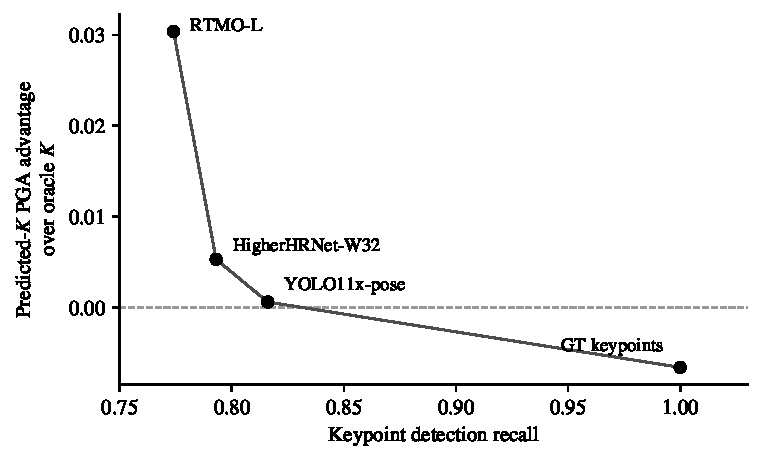
\includegraphics[width=0.75\linewidth]{figures/predk_recall.pdf}
    \caption{Difference in PGA between predicted-$K$ and oracle-$K$
    grouping as a function of keypoint recall for the three detector
    evaluations and the ground-truth-keypoint control. The predicted-$K$
    advantage increases across the three detector operating points as
    recall decreases, while the ground-truth-keypoint control reverses
    the effect when the input is complete. This pattern is consistent
    with the effective-person-count explanation -
    annotation-level $K$ becomes a less appropriate clustering
    constraint as the detected keypoint set becomes less complete.}
    \label{fig:predk_recall}
\end{figure}

The result also clarifies what the K-head's $76.1\%$ exact-count
accuracy does and does not measure.
That figure evaluates the prediction against the annotated number of
people,
whereas the downstream clustering problem operates only on the
keypoints that survived detection and matching.
A prediction counted as incorrect by the former criterion can therefore
still be useful to the latter.
The K-head is not outperforming an oracle estimate of the effective
person count -
rather, it can outperform the annotation-level count when that count
no longer describes the incomplete input to $k$-means.

The autonomous result should therefore not be interpreted as evidence
that estimated counts are generally preferable to known counts.
With complete observations, the ground-truth-keypoint control shows the
opposite.
The result is specific to the detector-based setting,
where the grouping module receives an incomplete representation of the
annotated scene.
In that setting, the predicted count acts as a form of calibration
to the available evidence.
This explains why the autonomous pipeline can slightly outperform the
oracle-$K$ diagnostic while also removing the final ground-truth
dependency from inference.


\subsection{Synthesis}
\label{sec_disc_modularity_autonomy_synthesis}

Reading Sections~\ref{sec_disc_modularity_autonomy_gap}
and~\ref{sec_disc_modularity_autonomy_autonomy} together gives a more
complete picture of the cost and benefit of separating grouping from
detection.
On HigherHRNet detections, the oracle-$K$ PG-GAT pipeline trails the
jointly trained AE reference by $0.0256$ PGA.
In return, the grouping network is no longer tied to the detector that
produced the keypoints.
The detector-swap experiments show that the same frozen PG-GAT
checkpoint can operate on HigherHRNet,
YOLO11x-pose,
and RTMO-L without retraining,
while remaining approximately $0.02$ PGA below each detector's native
grouping.
This is the experimental answer to \emph{RQ3: detector independence},
detector-independent grouping is achievable,
but it carries a small and measurable accuracy cost relative to
detector-specific grouping learned as part of the upstream model.

Whether this trade is worthwhile depends on the intended deployment
setting.
A fixed pipeline in which the detector and grouping mechanism can
always be trained and deployed together has little reason to give up
the additional accuracy of the native grouping method.
The modular design becomes useful when the grouping component must
remain reusable across detectors,
or when detection and grouping need to be developed,
updated,
or deployed independently.
Under those conditions, the approximately $0.020$--$0.022$ PGA
difference measured across the three detectors is the observed cost
of obtaining that flexibility.

The autonomous-pipeline result adds a second dimension to this finding.
Removing the ground-truth $K$ from the inference path might be expected
to introduce another accuracy penalty because errors made by the K-head
can propagate directly into $k$-means.
Instead, the predicted-$K$ HigherHRNet configuration reaches $0.9644$
PGA - compared with $0.9591$ for oracle $K$.
The detector-swap results show the same pattern,
with the predicted-$K$ advantage increasing as keypoint recall decreases.
The ground-truth-keypoint control reverses the effect when the input is
complete.
Taken together, these measurements support the effective-person-count
explanation developed in Section~\ref{sec_disc_modularity_autonomy_autonomy}.

This result changes the role of K estimation in the modular pipeline.
The K-head is not simply an imperfect replacement for information that
would ideally be supplied by an oracle.
In the detector-based setting,
the annotation-level person count and the number of people represented
by the available keypoints can differ.
The K-head operates on the detected representation and can therefore
adapt its prediction to the evidence that actually reaches the grouping
stage.
Its prediction can be wrong relative to the annotated person count
while still providing a better clustering constraint for the incomplete
detection set.

This provides the experimental answer to \emph{RQ7: autonomous
deployment}.
The final pipeline does not require ground-truth person counts at
inference,
and removing that dependency does not reduce the measured grouping
accuracy on the detector outputs tested here.
For HigherHRNet and RTMO-L it improves it measurably,
while for YOLO11x-pose the difference is close to neutral.
The ground-truth control is equally important to this conclusion -
it shows that predicted $K$ is not intrinsically superior to known $K$,
but becomes useful when detection errors create a mismatch between the
annotated scene and the evidence presented to the grouping algorithm.

The combined result is therefore stronger than the oracle-$K$
modularity experiment alone.
PG-GAT pays a modest accuracy cost to separate grouping from detection,
and the detector-swap experiments show that this separation is
operational across multiple detector families.
The K-head then removes the remaining ground-truth dependency without
introducing the expected additional penalty and,
under incomplete detection, can partially offset the oracle-$K$
grouping cost.
The contribution is consequently not that modularity is free,
but that its cost is measured,
stable across the detectors tested,
and compatible with a fully autonomous inference pipeline.
\section{Research Question Recap}
\label{sec_disc_rq_recap}

This closing section consolidates the answers to the seven research questions of Section~\ref{sec_intro_objective} for the reader's convenience.
The substantive arguments and evidence appear in Sections~\ref{sec_disc_embedding}--\ref{sec_disc_modularity_autonomy} of this chapter and the corresponding experimental sections of Chapter~\ref{chap_4};
the table below maps each question to its answer and the section in which the supporting evidence is developed.

\begingroup
\tablesize
\renewcommand{\arraystretch}{1.25}
\begin{longtable}{p{0.18\linewidth}p{0.55\linewidth}p{0.18\linewidth}}
\toprule
Research question & Answer & Evidence \\
\midrule
\endfirsthead
\toprule
Research question & Answer & Evidence \\
\midrule
\endhead
\midrule
\multicolumn{3}{r}{\emph{continued on next page}} \\
\endfoot
\bottomrule
\caption{Concise mapping of each research question to its answer and the discussion section in which the supporting argument is developed.
The substantive interpretation of each result appears in the referenced section;
this table is a navigation aid and not the substance of the chapter.}
\label{tab:rq_recap}
\endlastfoot
RQ1 --- The lever &
The binding constraint is the per-keypoint embedding, not the grouping algorithm.
Three learned heads and ten modularity variants all fail to outperform plain $k$-means on the standard embedding,
while embedding-side modifications are the only changes whose gains survive transfer to COCO.
& \S\ref{sec_disc_embedding_heads}, \S\ref{sec_disc_embedding_sadmon}, \S\ref{sec_disc_embedding_pggat} \\

RQ2 --- Inductive biases &
The three skeleton-aware modifications (type-pair attention, skeleton-relative positional encoding, same-type repulsion heads) each contribute approximately $+0.005$ in isolation and approximately $+0.011$ in combination.
The architecture sweep over depth and capacity dominates the modifications ($+0.0738$ over the ablation row).
The loss sweep produces no configuration above the defaults.
& \S\ref{sec_disc_embedding_pggat} \\

RQ3 --- Detector independence &
The modular grouper reaches $0.9591$ E2E PGA against HigherHRNet AE's $0.9847$ on the same matched detections,
a gap of $0.0256$.
Applied zero-shot to YOLO11x-pose and RTMO-L detections,
the autonomous pipeline trails each detector's native grouping by $0.0210$ and $0.0220$;
the price of detector independence is therefore stable at approximately $0.02$ PGA across three detector families.
& \S\ref{sec_disc_modularity_autonomy_gap}, \S\ref{sec_res_e2e_swap} \\

RQ4 --- Embedding geometry &
The hyperbolic variant matches the Euclidean variant at four-fold smaller embedding dimension under synthetic-only training (H2 supported)
but loses to the Euclidean variant by $0.0166$ COCO PGA after COCO fine-tuning.
Hyperbolic geometry is an efficiency observation at low dimension, not a quality win at the headline operating point.
H1 (quality at matched dimension) is unsupported.
& \S\ref{sec_disc_transfer_hyperbolic} \\

RQ5 --- Graph primitive &
The triplet primitive underperforms the joint primitive by $0.0156$ synth val PGA at matched training compute.
The dominant failure mode is the voting step that converts per-triplet cluster labels into per-joint labels;
small per-triplet errors propagate to multiple joint memberships.
The negative result is attributed to the triplet-to-joint voting stage
rather than to the articulation signal itself.
& \S\ref{sec_disc_transfer_trigat} \\

RQ6 --- Synthetic-to-real transfer &
COCO fine-tuning lifts the embedding by approximately $+0.07$ COCO val PGA at the architecture-sweep winner,
the single largest gain measured in the experimental chapter.
Synthetic-validation accuracy is preserved through fine-tuning (no catastrophic forgetting at the sweep operating point),
and the lift is comparable in magnitude to the entire architecture sweep.
& \S\ref{sec_disc_transfer_finetune} \\

RQ7 --- Autonomous deployment &
The K-head trained on the meng-headline COCO embeddings achieves $76.1\%$ exact K-prediction accuracy and $91.9\%$ off-by-one accuracy on COCO val.
The resulting autonomous pipeline produces $0.9644$ E2E PGA,
$0.0053$ \emph{above} the oracle-K row at $0.9591$.
The evidence is consistent with the K prediction calibrating to the effective person count in the matched-detection set,
whereas oracle K describes the annotated scene;
the advantage is monotone in the recall deficit across four operating points
($+0.0006$ to $+0.0304$ as recall falls from $0.816$ to $0.774$, with a sign flip at perfect recall).
The autonomous pipeline is therefore not a compromise relative to oracle K but the operational measurement of the complete system.
& \S\ref{sec_disc_modularity_autonomy_autonomy}, \S\ref{sec_res_e2e_swap} \\
\end{longtable}
\endgroup


%% End of File.
